\begin{frame}{Vector Similarity Search with FAISS}

\begin{columns}[T]
  \begin{column}{0.40\textwidth}
    \begin{itemize}
        \item Used \textbf{Facebook AI Similarity Search (FAISS)} library
        \item Performs \textbf{L2 distance} search in embedding space
        \item Index built with:
          \begin{itemize}
            \item 5160 book embeddings (\( \vec{v} \in \mathbb{R}^{384} \))
            \item Exact search (IndexFlatL2)
          \end{itemize}
        \item At runtime:
          \begin{itemize}
            \item User query is embedded
            \item Top-k nearest neighbors retrieved
            \item Results shown in UI
          \end{itemize}
        \item \textbf{Fully local}, fast search
    \end{itemize}
  \end{column}

  \begin{column}{0.55\textwidth}
    \centering
    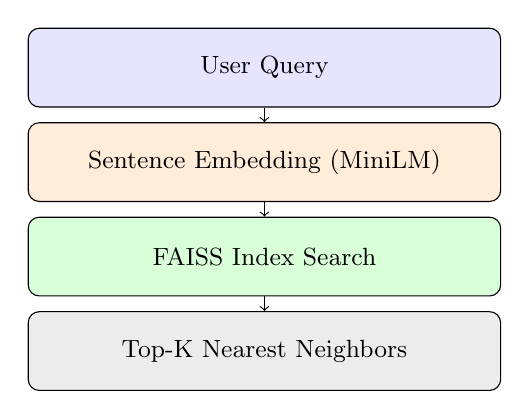
\begin{tikzpicture}[node distance=1.2cm, every node/.style={font=\small}]
        \node (query) [draw, rounded corners, minimum width=6cm, minimum height=1cm, fill=blue!10] {User Query};

        \node (embed) [below of=query, draw, rounded corners, minimum width=6cm, minimum height=1cm, fill=orange!15] {Sentence Embedding (MiniLM)};

        \node (faiss) [below of=embed, draw, rounded corners, minimum width=6cm, minimum height=1cm, fill=green!15] {FAISS Index Search};

        \node (results) [below of=faiss, draw, rounded corners, minimum width=6cm, minimum height=1cm, fill=gray!15] {Top-K Nearest Neighbors};

        \draw[->] (query) -- (embed);
        \draw[->] (embed) -- (faiss);
        \draw[->] (faiss) -- (results);
    \end{tikzpicture}
  \end{column}
\end{columns}

\end{frame}
